%! TEX encoding = utf8
\chapter{Regulacja z skokowym zakłóceniem sinusoidalnym}

W tym podpunkcie zakłócenie pojawia się w chwili k=60 i posiada ono charakter sinusoidalny.

\section{Bez pomiaru zakłócenia}

\begin{figure}[H]
\centering
% This file was created by matlab2tikz.
%
%The latest updates can be retrieved from
%  http://www.mathworks.com/matlabcentral/fileexchange/22022-matlab2tikz-matlab2tikz
%where you can also make suggestions and rate matlab2tikz.
%
\definecolor{mycolor1}{rgb}{0.00000,0.44700,0.74100}%
%
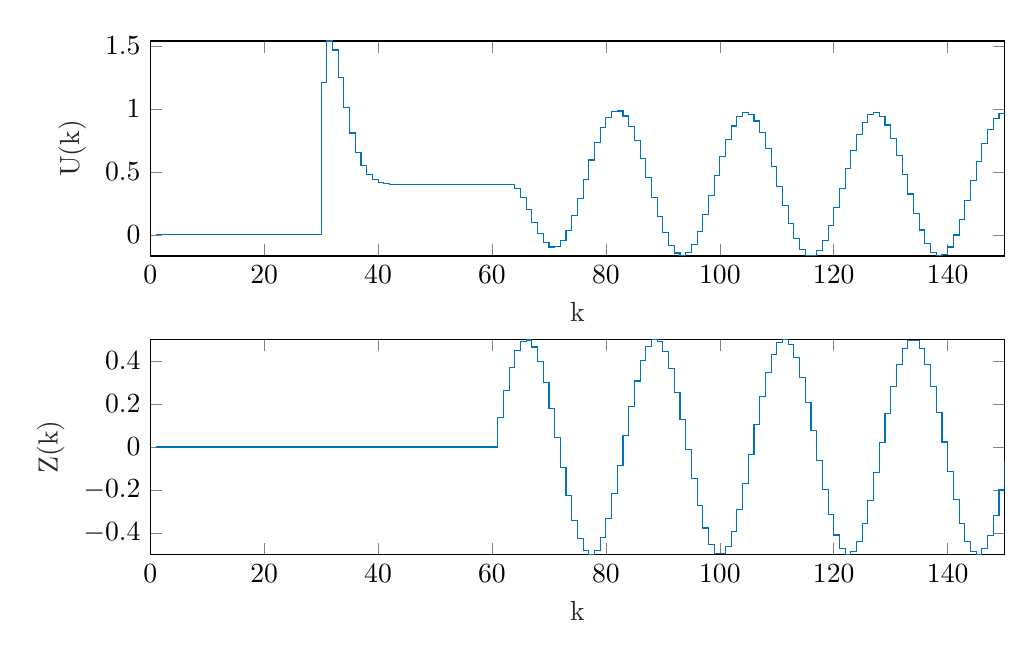
\begin{tikzpicture}

\begin{axis}[%
width=4.272in,
height=1.075in,
at={(0.717in,1.839in)},
scale only axis,
xmin=0,
xmax=150,
xlabel style={font=\color{white!15!black}},
xlabel={k},
ymin=-0.166609326859868,
ymax=1.538576433506,
ylabel style={font=\color{white!15!black}},
ylabel={U(k)},
axis background/.style={fill=white}
]
\addplot[const plot, color=mycolor1, forget plot] table[row sep=crcr] {%
1	0\\
2	0\\
3	0\\
4	0\\
5	0\\
6	0\\
7	0\\
8	0\\
9	0\\
10	0\\
11	0\\
12	0\\
13	0\\
14	0\\
15	0\\
16	0\\
17	0\\
18	0\\
19	0\\
20	0\\
21	0\\
22	0\\
23	0\\
24	0\\
25	0\\
26	0\\
27	0\\
28	0\\
29	0\\
30	1.20577393725138\\
31	1.538576433506\\
32	1.46712127199355\\
33	1.24868968296282\\
34	1.01114447937986\\
35	0.808413088923491\\
36	0.655593901391529\\
37	0.54975127059157\\
38	0.481347710796871\\
39	0.4399381217831\\
40	0.416581469792359\\
41	0.404525444762055\\
42	0.399086664830369\\
43	0.397234397851693\\
44	0.397131373389285\\
45	0.397739526004153\\
46	0.39852169972768\\
47	0.39923446155087\\
48	0.39979385972787\\
49	0.400193942132608\\
50	0.400460651022531\\
51	0.400627917253023\\
52	0.40072678887092\\
53	0.400781648510957\\
54	0.400809906317153\\
55	0.40082312096247\\
56	0.400828485130777\\
57	0.40083019020383\\
58	0.400830499953435\\
59	0.400830517872924\\
60	0.400830696699621\\
61	0.400831155277304\\
62	0.400831862848653\\
63	0.400832738153988\\
64	0.367435097102787\\
65	0.297730044122255\\
66	0.203403988540624\\
67	0.101390485220279\\
68	0.00865316048981549\\
69	-0.0605458871185013\\
70	-0.0959344027760143\\
71	-0.0916909796189358\\
72	-0.0464185959935534\\
73	0.0371931415874952\\
74	0.152927480323017\\
75	0.291770144407255\\
76	0.442767731529408\\
77	0.593970220173893\\
78	0.733405292823735\\
79	0.850025702457492\\
80	0.934568531419711\\
81	0.980268134743467\\
82	0.983372896403964\\
83	0.943428969198735\\
84	0.863310740495651\\
85	0.748996400777699\\
86	0.609106092740255\\
87	0.454238093762833\\
88	0.296153867174819\\
89	0.146874371085384\\
90	0.0177568170157902\\
91	-0.0813774171802304\\
92	-0.142996920768938\\
93	-0.162438658422041\\
94	-0.138266341734569\\
95	-0.0723813126568258\\
96	0.0301225449520763\\
97	0.161348729481161\\
98	0.311202977648383\\
99	0.46816667274684\\
100	0.620179504455711\\
101	0.755563704716845\\
102	0.863918997436818\\
103	0.936919645592213\\
104	0.968952485566794\\
105	0.957547029789689\\
106	0.903564660339399\\
107	0.811132405964747\\
108	0.687326376957459\\
109	0.541629125229492\\
110	0.385202529366831\\
111	0.230031947551548\\
112	0.088007250776386\\
113	-0.0299888119306022\\
114	-0.114915026505379\\
115	-0.160264935416994\\
116	-0.162565722553433\\
117	-0.121644515000728\\
118	-0.0406416863198654\\
119	0.0742298578755635\\
120	0.214160956892216\\
121	0.368421519852338\\
122	0.525183123813124\\
123	0.672425819673637\\
124	0.798859624639607\\
125	0.894790054106067\\
126	0.952861336109481\\
127	0.968620329077551\\
128	0.940857909528836\\
129	0.871701656806462\\
130	0.766452728922126\\
131	0.633179435355932\\
132	0.482098665656075\\
133	0.324792596866525\\
134	0.173320731277157\\
135	0.0392953405700984\\
136	-0.067009378456163\\
137	-0.137444144389846\\
138	-0.166609326859868\\
139	-0.152269079853141\\
140	-0.0955229009945729\\
141	-0.000721413095445669\\
142	0.124867163036136\\
143	0.271614248074047\\
144	0.428269113032137\\
145	0.582821449292206\\
146	0.723422164836795\\
147	0.839291812497467\\
148	0.921547006537011\\
149	0.963881472054508\\
150	0.963049516192931\\
};
\end{axis}

\begin{axis}[%
width=4.272in,
height=1.075in,
at={(0.717in,0.346in)},
scale only axis,
xmin=0,
xmax=150,
xlabel style={font=\color{white!15!black}},
xlabel={k},
ymin=-0.5,
ymax=0.5,
ylabel style={font=\color{white!15!black}},
ylabel={Z(k)},
axis background/.style={fill=white}
]
\addplot[const plot, color=mycolor1, forget plot] table[row sep=crcr] {%
1	0\\
2	0\\
3	0\\
4	0\\
5	0\\
6	0\\
7	0\\
8	0\\
9	0\\
10	0\\
11	0\\
12	0\\
13	0\\
14	0\\
15	0\\
16	0\\
17	0\\
18	0\\
19	0\\
20	0\\
21	0\\
22	0\\
23	0\\
24	0\\
25	0\\
26	0\\
27	0\\
28	0\\
29	0\\
30	0\\
31	0\\
32	0\\
33	0\\
34	0\\
35	0\\
36	0\\
37	0\\
38	0\\
39	0\\
40	0\\
41	0\\
42	0\\
43	0\\
44	0\\
45	0\\
46	0\\
47	0\\
48	0\\
49	0\\
50	0\\
51	0\\
52	0\\
53	0\\
54	0\\
55	0\\
56	0\\
57	0\\
58	0\\
59	0\\
60	0\\
61	0.137109644605363\\
62	0.263707692885933\\
63	0.370088426598019\\
64	0.448096100514978\\
65	0.491750207716154\\
66	0.497703978875882\\
67	0.465500964418924\\
68	0.397610028511525\\
69	0.299236072051978\\
70	0.177920995700533\\
71	0.0429654953665704\\
72	-0.0952839814377427\\
73	-0.226228452441949\\
74	-0.339828978196373\\
75	-0.42737630361942\\
76	-0.482158558464389\\
77	-0.499975827033521\\
78	-0.479462137331569\\
79	-0.422190184159834\\
80	-0.332550757489411\\
81	-0.217416119812539\\
82	-0.0856131398571169\\
83	0.0527534248035702\\
84	0.18707561528561\\
85	0.307055537171193\\
86	0.403494854999882\\
87	0.468999988387369\\
88	0.498548945471937\\
89	0.489876337049306\\
90	0.443647054047348\\
91	0.363405293248861\\
92	0.255302839237141\\
93	0.127627433998259\\
94	-0.00983260798168206\\
95	-0.146538826944862\\
96	-0.272010555444685\\
97	-0.376628425245164\\
98	-0.452371842179728\\
99	-0.493433889999937\\
100	-0.496666521227455\\
101	-0.461821904175253\\
102	-0.391571423118295\\
103	-0.291300874953792\\
104	-0.168697563726657\\
105	-0.0331609486756003\\
106	0.10491797116538\\
107	0.234953289381683\\
108	0.346975767288528\\
109	0.432397131825702\\
110	0.484668500862322\\
111	0.499782457325439\\
112	0.476580280326615\\
113	0.416840779220727\\
114	0.325143920078558\\
115	0.2085196997346\\
116	0.0759091866999565\\
117	-0.0625209514254677\\
118	-0.196157881858479\\
119	-0.314756246069852\\
120	-0.409223626578972\\
121	-0.472317622804679\\
122	-0.499201094217933\\
123	-0.487813002734079\\
124	-0.439026423481658\\
125	-0.356581609953743\\
126	-0.246799245143661\\
127	-0.118095862445442\\
128	0.019661413122442\\
129	0.155911334203973\\
130	0.280208215713932\\
131	0.383022759792753\\
132	0.456472625363814\\
133	0.494926732722869\\
134	0.49543697377182\\
135	0.45796423056276\\
136	0.385381374299828\\
137	0.283253014878502\\
138	0.159408886601137\\
139	0.0233435767186514\\
140	-0.114511383016329\\
141	-0.243587256230255\\
142	-0.353988360687203\\
143	-0.437250726932631\\
144	-0.486990993784778\\
145	-0.499395792696579\\
146	-0.473514102031107\\
147	-0.411330157727866\\
148	-0.317611330618286\\
149	-0.19954263297079\\
150	-0.0661758750488865\\
};
\end{axis}
\end{tikzpicture}%
\caption{Zakłócenie i sygnał sterujący}
\end{figure}

\begin{figure}[H]
\centering
% This file was created by matlab2tikz.
%
%The latest updates can be retrieved from
%  http://www.mathworks.com/matlabcentral/fileexchange/22022-matlab2tikz-matlab2tikz
%where you can also make suggestions and rate matlab2tikz.
%
\definecolor{mycolor1}{rgb}{0.00000,0.44700,0.74100}%
\definecolor{mycolor2}{rgb}{0.85000,0.32500,0.09800}%
%
\begin{tikzpicture}

\begin{axis}[%
width=4.272in,
height=2.472in,
at={(0.717in,0.441in)},
scale only axis,
xmin=0,
xmax=150,
xlabel style={font=\color{white!15!black}},
xlabel={k},
ymin=0,
ymax=2,
ylabel style={font=\color{white!15!black}},
ylabel={Y(k)},
axis background/.style={fill=white},
legend style={legend cell align=left, align=left, draw=white!15!black}
]
\addplot[const plot, color=mycolor1] table[row sep=crcr] {%
1	0\\
2	0\\
3	0\\
4	0\\
5	0\\
6	0\\
7	0\\
8	0\\
9	0\\
10	0\\
11	0\\
12	0\\
13	0\\
14	0\\
15	0\\
16	0\\
17	0\\
18	0\\
19	0\\
20	0\\
21	0\\
22	0\\
23	0\\
24	0\\
25	0\\
26	0\\
27	0\\
28	0\\
29	0\\
30	0\\
31	0\\
32	0\\
33	0\\
34	0\\
35	0\\
36	0\\
37	0.178309849840735\\
38	0.3952760141839\\
39	0.588826611204609\\
40	0.738611928918155\\
41	0.844395923345594\\
42	0.913931740693088\\
43	0.956746557749988\\
44	0.981369563669113\\
45	0.994414676921337\\
46	1.00055965866249\\
47	1.00288312467568\\
48	1.00328286848648\\
49	1.00285171378131\\
50	1.00216956244591\\
51	1.0015102513556\\
52	1.00097786168913\\
53	1.00059084702661\\
54	1.00033054211392\\
55	1.00016694785008\\
56	1.0000709398569\\
57	1.00001893584117\\
58	0.999993751094316\\
59	0.999983795371811\\
60	0.999981757686305\\
61	0.999983323334048\\
62	0.999986132468706\\
63	0.999989019847488\\
64	1.02769039166633\\
65	1.07785743800136\\
66	1.14388383488865\\
67	1.21825702710571\\
68	1.2930994268854\\
69	1.3607415194462\\
70	1.41428248576507\\
71	1.44315598097269\\
72	1.43834127875431\\
73	1.39481303289178\\
74	1.31233171988639\\
75	1.19526454819569\\
76	1.05185403895729\\
77	0.893184863574524\\
78	0.732005454196305\\
79	0.581511985029353\\
80	0.454178440083178\\
81	0.360704102732015\\
82	0.309140607678266\\
83	0.304250187548151\\
84	0.34713305902558\\
85	0.43514488245956\\
86	0.562105800870481\\
87	0.718782196695702\\
88	0.893602701398449\\
89	1.07355283515382\\
90	1.24517941697963\\
91	1.39562770943658\\
92	1.51363186161568\\
93	1.59038283185553\\
94	1.62020736608566\\
95	1.60100607935948\\
96	1.53441713853094\\
97	1.42569306380866\\
98	1.28330014654361\\
99	1.11827123530822\\
100	0.943361542209704\\
101	0.772072216871197\\
102	0.617616568715968\\
103	0.491908211752498\\
104	0.404648722787739\\
105	0.362584772692679\\
106	0.36899169590165\\
107	0.423423101866583\\
108	0.521745734670998\\
109	0.656456917183607\\
110	0.817260250636173\\
111	0.991855440326366\\
112	1.16688170125506\\
113	1.32894242251041\\
114	1.46563253883733\\
115	1.56648984972922\\
116	1.62379735649565\\
117	1.63317510912079\\
118	1.59391619169969\\
119	1.50904109066826\\
120	1.38506628009304\\
121	1.23150476774062\\
122	1.06013689479701\\
123	0.884107295539178\\
124	0.716917250624331\\
125	0.571389687206596\\
126	0.458686175987246\\
127	0.387451288793609\\
128	0.363149915988334\\
129	0.387648349519463\\
130	0.459071248883174\\
131	0.571945456452394\\
132	0.717619637065152\\
133	0.884927570462139\\
134	1.06104424530716\\
135	1.23246912221889\\
136	1.38606118370493\\
137	1.51004641857314\\
138	1.59492050168703\\
139	1.63417746481401\\
140	1.62480849478803\\
141	1.56753261851536\\
142	1.46674158939203\\
143	1.3301631153739\\
144	1.16826846252443\\
145	0.993469724082691\\
146	0.819168266989711\\
147	0.658727311975844\\
148	0.524447426927005\\
149	0.426623487371497\\
150	0.372755407745784\\
};
\addlegendentry{Y}

\addplot[const plot, color=mycolor2] table[row sep=crcr] {%
1	0\\
2	0\\
3	0\\
4	0\\
5	0\\
6	0\\
7	0\\
8	0\\
9	0\\
10	0\\
11	0\\
12	0\\
13	0\\
14	0\\
15	0\\
16	0\\
17	0\\
18	0\\
19	0\\
20	0\\
21	0\\
22	0\\
23	0\\
24	0\\
25	0\\
26	0\\
27	0\\
28	0\\
29	0\\
30	1\\
31	1\\
32	1\\
33	1\\
34	1\\
35	1\\
36	1\\
37	1\\
38	1\\
39	1\\
40	1\\
41	1\\
42	1\\
43	1\\
44	1\\
45	1\\
46	1\\
47	1\\
48	1\\
49	1\\
50	1\\
51	1\\
52	1\\
53	1\\
54	1\\
55	1\\
56	1\\
57	1\\
58	1\\
59	1\\
60	1\\
61	1\\
62	1\\
63	1\\
64	1\\
65	1\\
66	1\\
67	1\\
68	1\\
69	1\\
70	1\\
71	1\\
72	1\\
73	1\\
74	1\\
75	1\\
76	1\\
77	1\\
78	1\\
79	1\\
80	1\\
81	1\\
82	1\\
83	1\\
84	1\\
85	1\\
86	1\\
87	1\\
88	1\\
89	1\\
90	1\\
91	1\\
92	1\\
93	1\\
94	1\\
95	1\\
96	1\\
97	1\\
98	1\\
99	1\\
100	1\\
101	1\\
102	1\\
103	1\\
104	1\\
105	1\\
106	1\\
107	1\\
108	1\\
109	1\\
110	1\\
111	1\\
112	1\\
113	1\\
114	1\\
115	1\\
116	1\\
117	1\\
118	1\\
119	1\\
120	1\\
121	1\\
122	1\\
123	1\\
124	1\\
125	1\\
126	1\\
127	1\\
128	1\\
129	1\\
130	1\\
131	1\\
132	1\\
133	1\\
134	1\\
135	1\\
136	1\\
137	1\\
138	1\\
139	1\\
140	1\\
141	1\\
142	1\\
143	1\\
144	1\\
145	1\\
146	1\\
147	1\\
148	1\\
149	1\\
150	1\\
151	1\\
152	1\\
153	1\\
154	1\\
155	1\\
156	1\\
157	1\\
158	1\\
159	1\\
160	1\\
161	1\\
162	1\\
163	1\\
164	1\\
165	1\\
166	1\\
167	1\\
168	1\\
169	1\\
170	1\\
171	1\\
172	1\\
173	1\\
174	1\\
175	1\\
176	1\\
177	1\\
178	1\\
179	1\\
180	1\\
181	1\\
182	1\\
183	1\\
184	1\\
185	1\\
186	1\\
187	1\\
188	1\\
189	1\\
190	1\\
191	1\\
192	1\\
193	1\\
194	1\\
195	1\\
196	1\\
197	1\\
198	1\\
199	1\\
200	1\\
};
\addlegendentry{Yzad}

\end{axis}
\end{tikzpicture}%
\caption{Wyjście obiektu bez pomiaru zakłócenia błąd $E=24,84831$}
\end{figure}

\section{Z pomiaru zakłócenia}

\begin{figure}[H]
\centering
% This file was created by matlab2tikz.
%
%The latest updates can be retrieved from
%  http://www.mathworks.com/matlabcentral/fileexchange/22022-matlab2tikz-matlab2tikz
%where you can also make suggestions and rate matlab2tikz.
%
\definecolor{mycolor1}{rgb}{0.00000,0.44700,0.74100}%
%
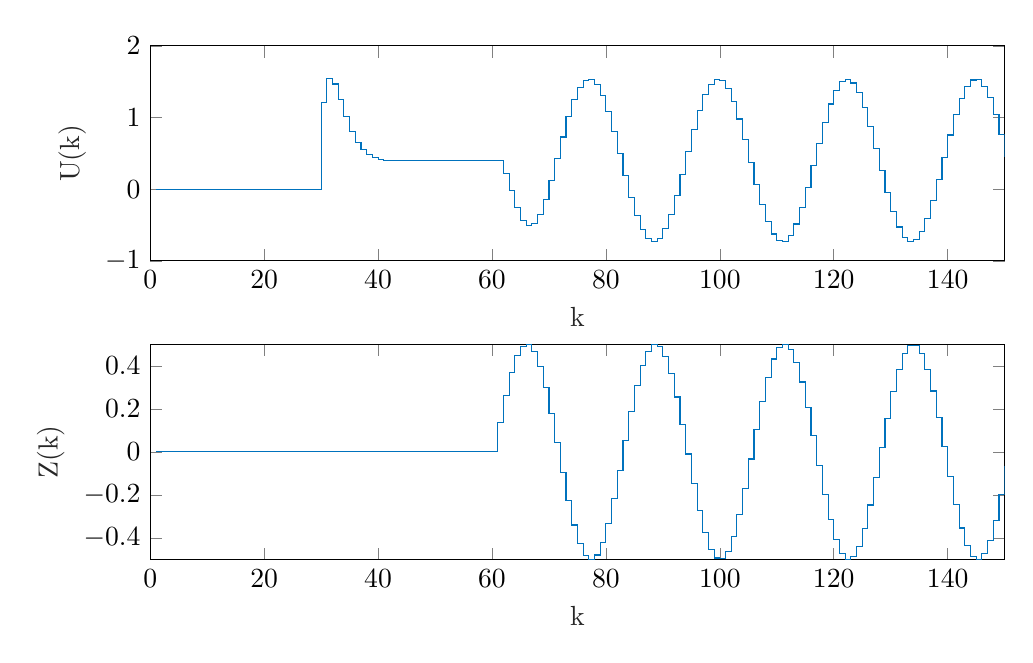
\begin{tikzpicture}

\begin{axis}[%
width=4.272in,
height=1.075in,
at={(0.717in,1.839in)},
scale only axis,
xmin=0,
xmax=150,
xlabel style={font=\color{white!15!black}},
xlabel={k},
ymin=-1,
ymax=2,
ylabel style={font=\color{white!15!black}},
ylabel={U(k)},
axis background/.style={fill=white}
]
\addplot[const plot, color=mycolor1, forget plot] table[row sep=crcr] {%
1	0\\
2	0\\
3	0\\
4	0\\
5	0\\
6	0\\
7	0\\
8	0\\
9	0\\
10	0\\
11	0\\
12	0\\
13	0\\
14	0\\
15	0\\
16	0\\
17	0\\
18	0\\
19	0\\
20	0\\
21	0\\
22	0\\
23	0\\
24	0\\
25	0\\
26	0\\
27	0\\
28	0\\
29	0\\
30	1.20577393725138\\
31	1.538576433506\\
32	1.46712127199355\\
33	1.24868968296282\\
34	1.01114447937986\\
35	0.808413088923491\\
36	0.655593901391529\\
37	0.54975127059157\\
38	0.481347710796871\\
39	0.4399381217831\\
40	0.416581469792359\\
41	0.404525444762055\\
42	0.399086664830369\\
43	0.397234397851693\\
44	0.397131373389285\\
45	0.397739526004153\\
46	0.39852169972768\\
47	0.39923446155087\\
48	0.39979385972787\\
49	0.400193942132608\\
50	0.400460651022531\\
51	0.400627917253023\\
52	0.40072678887092\\
53	0.400781648510957\\
54	0.400809906317153\\
55	0.40082312096247\\
56	0.400828485130777\\
57	0.40083019020383\\
58	0.400830499953435\\
59	0.400830517872924\\
60	0.400830696699621\\
61	0.400831155277304\\
62	0.214730931936116\\
63	-0.0209719488252652\\
64	-0.261258242951346\\
65	-0.434715866905037\\
66	-0.509650749060827\\
67	-0.478907538584464\\
68	-0.350427648576571\\
69	-0.141442094127147\\
70	0.125227025584843\\
71	0.423754825116161\\
72	0.727374254174172\\
73	1.01019482072664\\
74	1.24887136357004\\
75	1.42410114207103\\
76	1.52187227258951\\
77	1.5343718343118\\
78	1.4604739940638\\
79	1.30575692701852\\
80	1.08203440454642\\
81	0.806427531060781\\
82	0.500041267418505\\
83	0.186341701868472\\
84	-0.110644495236152\\
85	-0.36817212926802\\
86	-0.566520768776604\\
87	-0.690506070473708\\
88	-0.730643462048976\\
89	-0.683875015508064\\
90	-0.553803768946816\\
91	-0.350417494900499\\
92	-0.0893230539378438\\
93	0.209449999744718\\
94	0.522984861644475\\
95	0.827234268771864\\
96	1.09886396357205\\
97	1.31704150445857\\
98	1.46503328470617\\
99	1.53148732360446\\
100	1.51130348333472\\
101	1.40602439487602\\
102	1.2237171212523\\
103	0.978354629388285\\
104	0.688744489415335\\
105	0.377086932472301\\
106	0.0672728136227735\\
107	-0.216948033048525\\
108	-0.45378762354228\\
109	-0.625090242758656\\
110	-0.717724389757285\\
111	-0.72458953549515\\
112	-0.64516050966913\\
113	-0.485527781202747\\
114	-0.257930544509929\\
115	0.0201815920005123\\
116	0.327486378739589\\
117	0.640423597704431\\
118	0.935001311829598\\
119	1.18863521354944\\
120	1.38188005764232\\
121	1.49992043686788\\
122	1.53370660905627\\
123	1.48064829667128\\
124	1.34481326819556\\
125	1.13661394932857\\
126	0.872010317098401\\
127	0.571286831823425\\
128	0.257497479486403\\
129	-0.0453016806086217\\
130	-0.313896857917448\\
131	-0.527707290333239\\
132	-0.67034288448544\\
133	-0.730866226398202\\
134	-0.704633962737328\\
135	-0.593654109425586\\
136	-0.406433163791048\\
137	-0.157323170154385\\
138	0.134578739199714\\
139	0.446894435253014\\
140	0.755680433401633\\
141	1.03726358344798\\
142	1.27005605898663\\
143	1.43621047755091\\
144	1.52298824614022\\
145	1.52373622091257\\
146	1.43839680475392\\
147	1.27351237892131\\
148	1.04172373316157\\
149	0.760800951344707\\
150	0.45228105338619\\
};
\end{axis}

\begin{axis}[%
width=4.272in,
height=1.075in,
at={(0.717in,0.346in)},
scale only axis,
xmin=0,
xmax=150,
xlabel style={font=\color{white!15!black}},
xlabel={k},
ymin=-0.5,
ymax=0.5,
ylabel style={font=\color{white!15!black}},
ylabel={Z(k)},
axis background/.style={fill=white}
]
\addplot[const plot, color=mycolor1, forget plot] table[row sep=crcr] {%
1	0\\
2	0\\
3	0\\
4	0\\
5	0\\
6	0\\
7	0\\
8	0\\
9	0\\
10	0\\
11	0\\
12	0\\
13	0\\
14	0\\
15	0\\
16	0\\
17	0\\
18	0\\
19	0\\
20	0\\
21	0\\
22	0\\
23	0\\
24	0\\
25	0\\
26	0\\
27	0\\
28	0\\
29	0\\
30	0\\
31	0\\
32	0\\
33	0\\
34	0\\
35	0\\
36	0\\
37	0\\
38	0\\
39	0\\
40	0\\
41	0\\
42	0\\
43	0\\
44	0\\
45	0\\
46	0\\
47	0\\
48	0\\
49	0\\
50	0\\
51	0\\
52	0\\
53	0\\
54	0\\
55	0\\
56	0\\
57	0\\
58	0\\
59	0\\
60	0\\
61	0.137109644605363\\
62	0.263707692885933\\
63	0.370088426598019\\
64	0.448096100514978\\
65	0.491750207716154\\
66	0.497703978875882\\
67	0.465500964418924\\
68	0.397610028511525\\
69	0.299236072051978\\
70	0.177920995700533\\
71	0.0429654953665704\\
72	-0.0952839814377427\\
73	-0.226228452441949\\
74	-0.339828978196373\\
75	-0.42737630361942\\
76	-0.482158558464389\\
77	-0.499975827033521\\
78	-0.479462137331569\\
79	-0.422190184159834\\
80	-0.332550757489411\\
81	-0.217416119812539\\
82	-0.0856131398571169\\
83	0.0527534248035702\\
84	0.18707561528561\\
85	0.307055537171193\\
86	0.403494854999882\\
87	0.468999988387369\\
88	0.498548945471937\\
89	0.489876337049306\\
90	0.443647054047348\\
91	0.363405293248861\\
92	0.255302839237141\\
93	0.127627433998259\\
94	-0.00983260798168206\\
95	-0.146538826944862\\
96	-0.272010555444685\\
97	-0.376628425245164\\
98	-0.452371842179728\\
99	-0.493433889999937\\
100	-0.496666521227455\\
101	-0.461821904175253\\
102	-0.391571423118295\\
103	-0.291300874953792\\
104	-0.168697563726657\\
105	-0.0331609486756003\\
106	0.10491797116538\\
107	0.234953289381683\\
108	0.346975767288528\\
109	0.432397131825702\\
110	0.484668500862322\\
111	0.499782457325439\\
112	0.476580280326615\\
113	0.416840779220727\\
114	0.325143920078558\\
115	0.2085196997346\\
116	0.0759091866999565\\
117	-0.0625209514254677\\
118	-0.196157881858479\\
119	-0.314756246069852\\
120	-0.409223626578972\\
121	-0.472317622804679\\
122	-0.499201094217933\\
123	-0.487813002734079\\
124	-0.439026423481658\\
125	-0.356581609953743\\
126	-0.246799245143661\\
127	-0.118095862445442\\
128	0.019661413122442\\
129	0.155911334203973\\
130	0.280208215713932\\
131	0.383022759792753\\
132	0.456472625363814\\
133	0.494926732722869\\
134	0.49543697377182\\
135	0.45796423056276\\
136	0.385381374299828\\
137	0.283253014878502\\
138	0.159408886601137\\
139	0.0233435767186514\\
140	-0.114511383016329\\
141	-0.243587256230255\\
142	-0.353988360687203\\
143	-0.437250726932631\\
144	-0.486990993784778\\
145	-0.499395792696579\\
146	-0.473514102031107\\
147	-0.411330157727866\\
148	-0.317611330618286\\
149	-0.19954263297079\\
150	-0.0661758750488865\\
};
\end{axis}
\end{tikzpicture}%
\caption{Zakłócenie i sygnał sterujący}
\end{figure}

\begin{figure}[H]
\centering
\input{rysunki/podpunkt6_z_2.230000e+01.tex}
\caption{Wyjście obiektu z pomiarem zakłócenia błąd $E=22,30000$}
\end{figure}

\section{Wnioski}
Z powyższych przebiegów można stwierdzić, że w przypadku pomiaru zakłócenia sinusoidalnego regulator działa lepiej niż bez (współczynnik jakości regulacji z pomiarem zakłócenia wynosi E=22,30000, natomiast bez E=24,84831).

\smallskip

